% ch07_matplotlib.tex -- Matplotlib: Scientific Visualization
\chapter{Matplotlib --- Scientific Visualization}
\label{ch:matplotlib}

\begin{intuition}
``A picture is worth a thousand words,'' and in science, a graph is worth a thousand
data tables. Matplotlib\index{Matplotlib} is the reference library in Python
for creating publication-quality figures. Think of it as the
``digital graph paper'' of the modern scientist.
\end{intuition}

% ============================================================
\section{First plot: \py{plt.plot()}}
\index{plt.plot}

\begin{codeblock}[title=\textbf{Python}]
\begin{minted}{python}
import numpy as np
import matplotlib.pyplot as plt

x = np.linspace(0, 2 * np.pi, 200)
y_sin = np.sin(x)
y_cos = np.cos(x)

plt.plot(x, y_sin, label="sin(x)")
plt.plot(x, y_cos, label="cos(x)", linestyle="--")
plt.xlabel("x (radians)")
plt.ylabel("y")
plt.title("Trigonometric functions")
plt.legend()
plt.grid(True)
plt.show()
\end{minted}
\end{codeblock}

\begin{codeoutput}
\begin{verbatim}
[Figure displayed: two curves sin(x) and cos(x) on [0, 2pi],
with legend, grid, and axis labels.]
\end{verbatim}
\end{codeoutput}

\begin{remark}
The convention is to import \py{matplotlib.pyplot as plt}. All plotting
functions are then accessible via \py{plt.function\_name()}.
\end{remark}

% --- TikZ anatomy of a figure ---
\begin{figure}[ht]
\centering
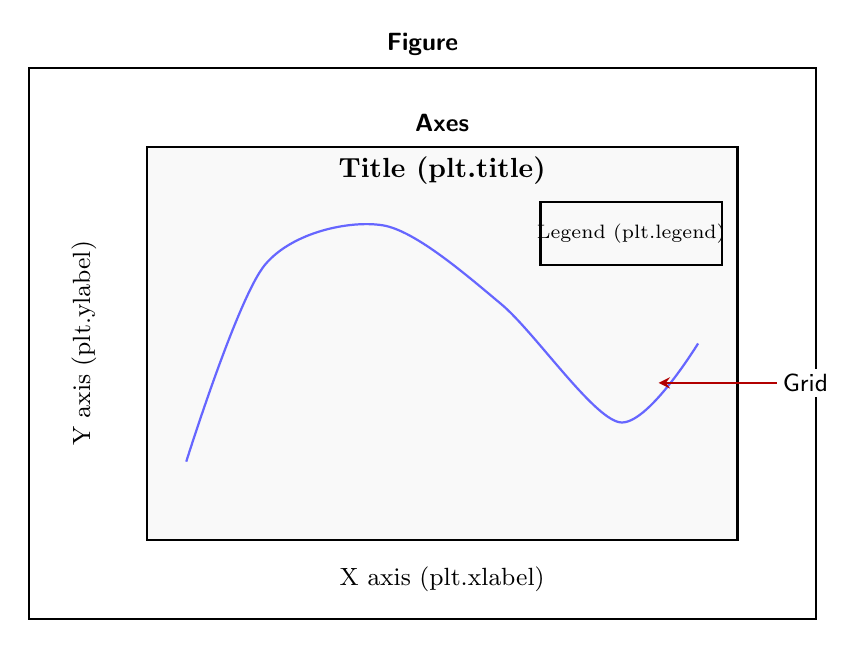
\begin{tikzpicture}[
    zone/.style={rectangle, draw, dashed, rounded corners},
    lbl/.style={font=\small\sffamily, fill=white, inner sep=2pt},
    arr/.style={->, thick, >=stealth, red!70!black}
]
% Figure frame
\draw[thick] (0,0) rectangle (10,7);
\node[lbl] at (5, 7.3) {\textbf{Figure}};

% Axes area
\draw[thick, fill=gray!5] (1.5, 1) rectangle (9, 6);
\node[lbl] at (5.25, 6.3) {\textbf{Axes}};

% Title
\node[font=\bfseries] at (5.25, 5.7) {Title (\py{plt.title})};

% Fake curve
\draw[blue!60, thick, smooth] plot coordinates
    {(2,2) (3,4.5) (4.5,5) (6,4) (7.5,2.5) (8.5,3.5)};

% X label
\node[font=\small] at (5.25, 0.5) {X axis (\py{plt.xlabel})};

% Y label
\node[font=\small, rotate=90] at (0.7, 3.5) {Y axis (\py{plt.ylabel})};

% Legend box
\draw[thick] (6.5, 4.5) rectangle (8.8, 5.3);
\node[font=\scriptsize] at (7.65, 4.9) {Legend (\py{plt.legend})};

% Grid annotation
\draw[arr] (9.5, 3) -- (8, 3);
\node[lbl, right] at (9.5, 3) {Grid};
\end{tikzpicture}
\caption{Anatomy of a Matplotlib figure: figure, axes, title, labels, and legend.}
\label{fig:matplotlib-anatomie}
\end{figure}

% ============================================================
\section{Scatter plots: \py{plt.scatter()}}
\index{plt.scatter}

\begin{codeblock}[title=\textbf{Python}]
\begin{minted}{python}
import numpy as np
import matplotlib.pyplot as plt

# Simulate experimental data
rng = np.random.default_rng(42)
n = 50
concentration = rng.uniform(0, 10, n)
absorbance = 0.42 * concentration + rng.normal(0, 0.3, n)

plt.scatter(concentration, absorbance, color="blue", alpha=0.6,
            label="Measurements")

# Regression line
coeffs = np.polyfit(concentration, absorbance, 1)
x_fit = np.linspace(0, 10, 100)
plt.plot(x_fit, np.polyval(coeffs, x_fit), "r-",
         label=f"Regression: y = {coeffs[0]:.2f}x + {coeffs[1]:.2f}")

plt.xlabel("Concentration (mol/L)")
plt.ylabel("Absorbance")
plt.title("Beer-Lambert Law")
plt.legend()
plt.grid(True, alpha=0.3)
plt.show()
\end{minted}
\end{codeblock}

\begin{codeoutput}
\begin{verbatim}
[Figure displayed: blue scatter points with red regression line,
title "Beer-Lambert Law", labeled axes.]
\end{verbatim}
\end{codeoutput}

% ============================================================
\section{Histograms: \py{plt.hist()}}
\index{plt.hist}

\begin{codeblock}[title=\textbf{Python}]
\begin{minted}{python}
import numpy as np
import matplotlib.pyplot as plt

rng = np.random.default_rng(42)

# Mass distribution of a sample
masses = rng.normal(loc=75, scale=8, size=1000)

plt.hist(masses, bins=30, color="green", alpha=0.7,
         edgecolor="black", density=True)
plt.xlabel("Mass (kg)")
plt.ylabel("Probability density")
plt.title("Mass distribution (n = 1000)")
plt.axvline(np.mean(masses), color="red", linestyle="--",
            label=f"Mean = {np.mean(masses):.1f} kg")
plt.legend()
plt.show()
\end{minted}
\end{codeblock}

\begin{codeoutput}
\begin{verbatim}
[Figure displayed: green histogram with 30 bars,
dashed red line marking the mean.]
\end{verbatim}
\end{codeoutput}

% ============================================================
\section{Bar charts: \py{plt.bar()}}
\index{plt.bar}

\begin{codeblock}[title=\textbf{Python}]
\begin{minted}{python}
import matplotlib.pyplot as plt

elements = ["H", "C", "N", "O", "S"]
abondance = [63.0, 9.5, 1.4, 25.5, 0.6]  # % in the human body

plt.bar(elements, abondance, color=["red", "gray", "blue",
        "cyan", "yellow"], edgecolor="black")
plt.xlabel("Chemical element")
plt.ylabel("Abundance (%)")
plt.title("Elemental composition of the human body")
plt.show()
\end{minted}
\end{codeblock}

\begin{codeoutput}
\begin{verbatim}
[Figure displayed: colored bar chart showing
the abundance of elements in the human body.]
\end{verbatim}
\end{codeoutput}

% ============================================================
\section{Subplots: \py{plt.subplots()}}
\index{subplots}

\begin{codeblock}[title=\textbf{Python}]
\begin{minted}{python}
import numpy as np
import matplotlib.pyplot as plt

x = np.linspace(0, 4 * np.pi, 300)

fig, axes = plt.subplots(2, 2, figsize=(10, 8))

# sin(x)
axes[0, 0].plot(x, np.sin(x), color="blue")
axes[0, 0].set_title("sin(x)")
axes[0, 0].grid(True)

# cos(x)
axes[0, 1].plot(x, np.cos(x), color="red")
axes[0, 1].set_title("cos(x)")
axes[0, 1].grid(True)

# exp(-x/5) * sin(x) -- damped signal
axes[1, 0].plot(x, np.exp(-x / 5) * np.sin(x), color="green")
axes[1, 0].set_title("Damped signal")
axes[1, 0].grid(True)

# x^2 and x^3
axes[1, 1].plot(x, x**2, label="$x^2$")
axes[1, 1].plot(x, x**3 / 10, label="$x^3/10$")
axes[1, 1].set_title("Polynomials")
axes[1, 1].legend()
axes[1, 1].grid(True)

plt.tight_layout()
plt.show()
\end{minted}
\end{codeblock}

\begin{codeoutput}
\begin{verbatim}
[Figure displayed: 2x2 grid of subplots with
sin(x), cos(x), damped signal, and polynomials.]
\end{verbatim}
\end{codeoutput}

\begin{bestpractice}
Always use \py{plt.tight\_layout()} or \py{fig.tight\_layout()} to prevent
labels from overlapping between subplots.
\end{bestpractice}

% ============================================================
\section{Advanced customization}
\index{customization}

\begin{codeblock}[title=\textbf{Python}]
\begin{minted}{python}
import numpy as np
import matplotlib.pyplot as plt

t = np.linspace(0, 10, 500)
y1 = np.sin(2 * np.pi * 0.5 * t)
y2 = np.sin(2 * np.pi * 1.0 * t)

plt.figure(figsize=(10, 5))
plt.plot(t, y1, "b-", linewidth=2, label="f = 0.5 Hz")
plt.plot(t, y2, "r--", linewidth=1.5, label="f = 1.0 Hz")

plt.xlabel("Time (s)", fontsize=14)
plt.ylabel("Amplitude", fontsize=14)
plt.title("Sinusoidal signals", fontsize=16, fontweight="bold")
plt.legend(fontsize=12, loc="upper right")
plt.xlim(0, 10)
plt.ylim(-1.5, 1.5)
plt.grid(True, alpha=0.3)

# Annotation
plt.annotate("Maximum", xy=(0.5, 1), xytext=(2, 1.3),
             arrowprops=dict(arrowstyle="->"), fontsize=11)

plt.show()
\end{minted}
\end{codeblock}

\begin{codeoutput}
\begin{verbatim}
[Figure displayed: two sinusoidal signals with different styles,
arrow annotation pointing to the maximum.]
\end{verbatim}
\end{codeoutput}

% ============================================================
\section{Saving a figure: \py{plt.savefig()}}
\index{plt.savefig}

\begin{codeblock}[title=\textbf{Python}]
\begin{minted}{python}
import numpy as np
import matplotlib.pyplot as plt

x = np.linspace(-5, 5, 200)
y = np.exp(-x**2 / 2) / np.sqrt(2 * np.pi)

plt.plot(x, y, "k-", linewidth=2)
plt.fill_between(x, y, alpha=0.3)
plt.xlabel("x")
plt.ylabel("f(x)")
plt.title("Standard normal distribution")

# Save in high resolution
plt.savefig("gaussienne.png", dpi=300, bbox_inches="tight")
plt.savefig("gaussienne.pdf", bbox_inches="tight")
print("Figure saved in PNG and PDF.")
\end{minted}
\end{codeblock}

\begin{codeoutput}
\begin{verbatim}
Figure saved in PNG and PDF.
\end{verbatim}
\end{codeoutput}

\begin{warning}
Call \py{plt.savefig()} \textbf{before} \py{plt.show()}, otherwise the figure will be
empty when saved. The option \py{bbox\_inches="tight"} prevents labels from being
clipped.
\end{warning}

% ============================================================
\section{Scientific figures: projectile trajectory}

\begin{codeblock}[title=\textbf{Python}]
\begin{minted}{python}
import numpy as np
import matplotlib.pyplot as plt

g = 9.81
angles = [30, 45, 60, 75]  # degrees
v0 = 20  # m/s

plt.figure(figsize=(10, 6))

for theta_deg in angles:
    theta = np.radians(theta_deg)
    t_vol = 2 * v0 * np.sin(theta) / g
    t = np.linspace(0, t_vol, 200)
    x = v0 * np.cos(theta) * t
    y = v0 * np.sin(theta) * t - 0.5 * g * t**2
    plt.plot(x, y, linewidth=2, label=f"theta = {theta_deg} deg")

plt.xlabel("Horizontal distance (m)", fontsize=13)
plt.ylabel("Height (m)", fontsize=13)
plt.title("Projectile trajectory (v0 = 20 m/s)", fontsize=14)
plt.legend(fontsize=11)
plt.grid(True, alpha=0.3)
plt.ylim(bottom=0)
plt.show()
\end{minted}
\end{codeblock}

\begin{codeoutput}
\begin{verbatim}
[Figure displayed: four parabolic trajectories for different
launch angles, showing that 45 deg gives the maximum range.]
\end{verbatim}
\end{codeoutput}

% ============================================================
\section{Common errors}

\begin{errmark}
\begin{enumerate}
    \item \textbf{Forgetting \py{plt.show()}}: in a script (outside Jupyter), without
    \py{plt.show()}, no window appears. The figure is created in memory
    but remains invisible.

    \item \textbf{Wrong figure size}: by default, figures are small.
    Use \py{plt.figure(figsize=(width, height))} to control the size
    in inches.

    \item \textbf{Saving after \py{plt.show()}}: \py{plt.show()} clears the current
    figure. Any call to \py{plt.savefig()} afterwards will produce an empty file.

    \item \textbf{Confusing \py{plt.plot} and the object-oriented interface}: for
    subplots, use \py{ax.plot()} rather than \py{plt.plot()} which acts on
    the last active axes.

    \item \textbf{Forgetting labels}: a graph without a title or axis labels
    is unusable in a scientific context. \emph{Always} add
    \py{xlabel}, \py{ylabel}, and \py{title}.
\end{enumerate}
\end{errmark}

% ============================================================
\section{Mini-project: Projectile Motion Visualization}

\begin{projet}
Create a complete program that:
\begin{enumerate}
    \item Asks for the initial velocity $v_0$ and the launch angle $\theta$.
    \item Computes the trajectory, range, and maximum height.
    \item Produces a figure with:
    \begin{itemize}
        \item The parabolic trajectory.
        \item A marked point at the apex (maximum height).
        \item An annotation indicating the range.
        \item A text box with the parameters ($v_0$, $\theta$, range, $h_{\max}$).
    \end{itemize}
    \item Saves the figure as a PDF.
\end{enumerate}
\end{projet}

\begin{codeblock}[title=\textbf{Python}]
\begin{minted}{python}
import numpy as np
import matplotlib.pyplot as plt

v0 = 25.0       # m/s
theta_deg = 55   # degrees
g = 9.81

theta = np.radians(theta_deg)
t_vol = 2 * v0 * np.sin(theta) / g
portee = v0**2 * np.sin(2 * theta) / g
h_max = (v0 * np.sin(theta))**2 / (2 * g)
t_max = v0 * np.sin(theta) / g

t = np.linspace(0, t_vol, 300)
x = v0 * np.cos(theta) * t
y = v0 * np.sin(theta) * t - 0.5 * g * t**2

fig, ax = plt.subplots(figsize=(10, 6))
ax.plot(x, y, "b-", linewidth=2.5)
ax.plot(v0 * np.cos(theta) * t_max, h_max, "ro", markersize=10)
ax.annotate(f"Apex\n({h_max:.1f} m)",
            xy=(v0 * np.cos(theta) * t_max, h_max),
            xytext=(portee * 0.6, h_max * 0.95),
            arrowprops=dict(arrowstyle="->"), fontsize=11)

info = (f"v0 = {v0} m/s\n"
        f"theta = {theta_deg} deg\n"
        f"Range = {portee:.1f} m\n"
        f"h_max = {h_max:.1f} m")
ax.text(0.02, 0.95, info, transform=ax.transAxes,
        fontsize=11, verticalalignment="top",
        bbox=dict(boxstyle="round", facecolor="wheat", alpha=0.8))

ax.set_xlabel("Distance (m)", fontsize=13)
ax.set_ylabel("Height (m)", fontsize=13)
ax.set_title("Projectile trajectory", fontsize=15)
ax.set_ylim(bottom=0)
ax.grid(True, alpha=0.3)
plt.tight_layout()
plt.savefig("projectile.pdf", bbox_inches="tight")
plt.show()
print(f"Range: {portee:.1f} m, Max height: {h_max:.1f} m")
\end{minted}
\end{codeblock}

\begin{codeoutput}
\begin{verbatim}
Range: 59.2 m, Max height: 21.4 m
\end{verbatim}
\end{codeoutput}

% ============================================================
\section{Exercises}

\begin{exercise}[$\star$ --- Exponential Curve]
Plot the function $f(x) = e^{-x/3} \cos(2\pi x)$ on $[0, 10]$.
Add a title, axis labels, and a grid.
\end{exercise}

\begin{exercise}[$\star$ --- Dice Roll Histogram]
Simulate 10,000 rolls of two dice. Plot the histogram of the sum obtained.
Which sum is the most frequent?
\end{exercise}

\begin{exercise}[$\star\star$ --- Phase Diagram]
Plot a simplified phase diagram of water: pressure ($y$) as a function of
temperature ($x$). Use \py{plt.fill\_between} to color the solid,
liquid, and gas regions.
\end{exercise}

\begin{exercise}[$\star\star$ --- Multiple Subplots]
Create a $2\times 2$ figure showing: (a) $\sin(x)$, (b) $\cos(x)$,
(c) $\tan(x)$ (limited to $[-5, 5]$), (d) $e^x$ and $\ln(x)$.
Each subplot must have its own title and grid.
\end{exercise}

\begin{exercise}[$\star\star\star$ --- Heatmap]
Create a $20\times 20$ matrix representing the temperature of a
hot plate (cold edges at 0\,\textdegree C, hot center at 100\,\textdegree C).
Display it with \py{plt.imshow()} and add a color bar.
\emph{Hint:} initialize a matrix of zeros and add a centered Gaussian.
\end{exercise}

% ============================================================
\begin{keyformulas}{Chapter Summary: Matplotlib}
\begin{itemize}
    \item \textbf{Curves}: \py{plt.plot(x, y, style, label=...)}
    \item \textbf{Scatter}: \py{plt.scatter(x, y, color=..., alpha=...)}
    \item \textbf{Histograms}: \py{plt.hist(data, bins=..., density=True)}
    \item \textbf{Bars}: \py{plt.bar(categories, values)}
    \item \textbf{Subplots}: \py{fig, axes = plt.subplots(nrows, ncols)}
    \item \textbf{Labels}: \py{plt.xlabel}, \py{plt.ylabel}, \py{plt.title}
    \item \textbf{Legend}: \py{plt.legend()} (after using \py{label=...})
    \item \textbf{Grid}: \py{plt.grid(True)}
    \item \textbf{Save}: \py{plt.savefig("name.pdf", dpi=300, bbox\_inches="tight")}
    \item \textbf{Golden rule}: \py{savefig} \emph{before} \py{show}
\end{itemize}
\end{keyformulas}
